%%%%%%%%%%%%%%%%%%%%%%%%%%%%%%%%%%%%%%%%
% Beamer Presentation
% LaTeX Template
% Version 1.0 (10/11/12)
%
% This template has been downloaded from:
% http://www.LaTeXTemplates.com
%
% License:
% CC BY-NC-SA 3.0 (http://creativecommons.org/licenses/by-nc-sa/3.0/)
%
%%%%%%%%%%%%%%%%%%%%%%%%%%%%%%%%%%%%%%%%%

%------------------------------------------------------------------------------%
%	PACKAGES AND THEMES
%------------------------------------------------------------------------------%

\documentclass{beamer}

\mode<presentation> {

% The Beamer class comes with a number of default slide themes
% which change the colors and layouts of slides. Below this is a list
% of all the themes, uncomment each in turn to see what they look like.

%\usetheme{default}
%\usetheme{AnnArbor}
%\usetheme{Antibes}
%\usetheme{Bergen}
%\usetheme{Berkeley}
%\usetheme{Berlin}
%\usetheme{Boadilla}
%\usetheme{CambridgeUS}
%\usetheme{Copenhagen}
%\usetheme{Darmstadt}
%\usetheme{Dresden}
%\usetheme{Frankfurt}
%\usetheme{Goettingen}
%\usetheme{Hannover}
%\usetheme{Ilmenau}
%\usetheme{JuanLesPins}
%\usetheme{Luebeck}
\usetheme{Madrid}
%\usetheme{Malmoe}
%\usetheme{Marburg}
%\usetheme{Montpellier}
%\usetheme{PaloAlto}
%\usetheme{Pittsburgh}
%\usetheme{Rochester}
%\usetheme{Singapore}
%\usetheme{Szeged}
%\usetheme{Warsaw}

% As well as themes, the Beamer class has a number of color themes
% for any slide theme. Uncomment each of these in turn to see how it
% changes the colors of your current slide theme.

%\usecolortheme{albatross}
%\usecolortheme{beaver}
%\usecolortheme{beetle}
%\usecolortheme{crane}
%\usecolortheme{dolphin}
%\usecolortheme{dove}
%\usecolortheme{fly}
%\usecolortheme{lily}
%\usecolortheme{orchid}
%\usecolortheme{rose}
%\usecolortheme{seagull}
%\usecolortheme{seahorse}
%\usecolortheme{whale}
%\usecolortheme{wolverine}

% To remove the footer line in all slides, uncomment this line
%\setbeamertemplate{footline}

% To replace the footer line in all slides with a simple slide count,
% uncomment this line
%\setbeamertemplate{footline}[page number]

% To remove the navigation symbols from the bottom of all slides,
% uncomment this line
\setbeamertemplate{navigation symbols}{}
}

% Allows including images
\usepackage{graphicx}

\usepackage[utf8]{inputenc}
\usepackage{multimedia}

% Allows the use of \toprule, \midrule and \bottomrule in tables
\usepackage{booktabs}

\usepackage{duckuments}

\usepackage{aasmacros}
%\usepackage[round,sort,numbers,authoryear]{natbib}
\bibliographystyle{apalike}

\usepackage{wasysym}

\usepackage{cancel}

\usepackage{tikz}

\definecolor{black}{RGB}{0,0,0}
\definecolor{caltechorange}{RGB}{242,84,34}
\setbeamercolor{palette primary}{bg=caltechorange,fg=white}
%\setbeamercolor{palette secondary}{bg=black,fg=white}
%\setbeamercolor{palette tertiary}{bg=black,fg=white}
\setbeamercolor{palette quaternary}{bg=black,fg=white}
\setbeamercolor{structure}{fg=black}
\setbeamercolor{section in toc}{fg=black}
\setbeamercolor{author in head/foot}{bg=caltechorange}
\setbeamercolor{title in head/foot}{bg=black}
\usepackage[font={color=black},figurename=Figure,bf]{caption}
\setbeamercolor{normal text}{fg=black}

\usefonttheme[onlymath]{serif}

% https://tex.stackexchange.com/questions/33969/changing-font-size-of-selected-slides-in-beamer
\newcommand\Fontvi{\fontsize{8}{8.2}\selectfont}
\newcommand\Fontvii{\fontsize{6}{6.2}\selectfont}

\usepackage{appendixnumberbeamer}
\usepackage{animate}

% Aliases
\newcommand{\amrex}{AMReX}
\newcommand{\ul}{\underline}
\newcommand{\p}{\partial}
\newcommand{\pd}[2]{\frac{\partial#1}{\partial#2}}
\newcommand{\bs}{\boldsymbol}
\newcommand{\red}{\textcolor{red}}
\newcommand{\mc}{\mathcal}
\newcommand{\rhoq}{\rho_{\mathrm{q}}}
\newcommand{\dvb}{\delta_{\mathrm{VB}}}


% --- TITLE PAGE SLIDE ---

\title[SXS Group Meeting]{14-Moment-Inspired Visco-Resistive MHD}

\author{Samuel J. Dunham}
\date{July 21, 2025}

\begin{document}

\begin{frame}

  \maketitle

\end{frame}

\begin{frame}
\frametitle{Physical Model}

  Baryon number, momentum, and energy are conserved:

  \begin{align}
    \nabla_{\mu} \, N^{\mu} &= 0 \, , \\
    \nabla_{\mu} \, T^{\mu\nu} &= 0 \, ,
  \end{align}
  where
  \begin{equation}
    T^{\mu\nu} = T^{\mu\nu}_{\mathrm{hydro}}
    + T^{\mu\nu}_{\mathrm{dissipative}} + T^{\mu\nu}_{\mathrm{EM}} \, .
  \end{equation}

  How to define $N^{\mu}$ and $T^{\mu\nu}_{\mathrm{hydro}}$, etc.?

\end{frame}

\begin{frame}
\frametitle{Viscous Hydrodynamics}

  Fluid-frame projector: $\Delta^{\mu\nu} := g^{\mu\nu} + u^{\mu} \, u^{\nu}$ \newline

  Decompose momentum into components parallel and perpendicular to four-velocity:
  $p^{\mu} = E_{\bs{p}} \, u^{\mu} + p^{\left<\mu\right>}$, with
  $p^{\left<\mu\right>} := \Delta^{\mu}_{~\nu} \, p^{\nu}$

  \begin{align}
    N^{\mu} &= n \, u^{\mu} + \red{n^{\mu}} \\
    T^{\mu\nu} &= \left( \rho + \rho \, \epsilon \right)
    u^{\mu} \, u^{\nu} + P \, \Delta^{\mu\nu} \notag \\
    &\ + \red{\Pi \, \Delta^{\mu\nu}
    + q^{\mu} \, u^{\nu} + q^{\nu} \, u^{\mu} + \pi^{\mu\nu}} \notag \\
    &\ + T^{\mu\nu}_{\mathrm{EM}} \, ,
  \end{align}
  where
  \begin{align}
    T^{\mu\nu}_{\mathrm{EM}}
    &:= \frac{1}{4\pi} \left( F^{\mu\alpha} \, F_{\alpha}^{~\nu}
    - \frac{1}{4} \, g^{\mu\nu} \, F^{\alpha\beta} \, F_{\alpha\beta} \right) \\
    &\phantom{:}= \frac{1}{2} \left( u^{\mu} \, u^{\nu} + \Delta^{\mu\nu} \right)
    \left( e_{\alpha} \, e^{\alpha} + b_{\alpha} \, b^{\alpha} \right)
    - 2 \, u^{\left(\mu\right.}b^{\left.\nu\right)\alpha} \, e_{\alpha}
    - \left( e^{\mu} \, e^{\nu} + b^{\mu} \, b^{\nu} \right)
  \end{align}

\end{frame}

\begin{frame}
\frametitle{Resistive Magnetohydrodynamics}

  \begin{equation}
    \nabla_{\mu} \, \mc{J}^{\mu} = 0
  \end{equation}
  \begin{equation}
    \mc{J}^{\mu} := \rhoq \, u^{\mu} + \red{J^{\mu}}
  \end{equation}
  \begin{equation}
    \nabla_{\nu} \left( J^{\mu} \, u^{\nu} \right)
    = -\frac{1}{\tau} \left( J^{\mu} - \eta^{-1} \, e^{\mu} \right)
    + \frac{\dvb}{\tau} \, \sqrt{b^{2}} \, b^{\mu\nu} \, J_{\nu}
  \end{equation}
\end{frame}

\begin{frame}
\frametitle{Evolution Equations}

  \begin{align}
    &\nabla_{\mu} \left[ \left( \Pi + \frac{\zeta}{\tau_{\Pi}} \right) u^{\mu} \right]
    = S_{\Pi} \\
    &\nabla_{\mu} \left[ q_{\nu} \, u^{\mu} + \frac{\kappa}{\tau_{\mathrm{q}}} \, T \, \Delta^{\mu}_{~\nu} \right]
    = \left(S_{\mathrm{q}}\right)_{\nu} \\
    &\nabla_{\mu} \left[ \pi^{\alpha\beta} \, u^{\mu}
    + 2 \, \frac{\eta}{\tau_{\pi}} \, g^{\mu\left(\alpha\right.}u^{\left.\beta\right)} \right]
    = \left(S_{\pi}\right)^{\alpha\beta} \\
    &\nabla_{\mu} \left[ J_{\nu} \, u^{\mu} \right]
    = \left(S_{\mathrm{J}}\right)_{\nu}
  \end{align}

\end{frame}

\begin{frame}
\frametitle{Primitive Variable Recovery}

  \begin{align}
    V = \left( \rho,
          W v^{i},
          e, 
          B^{i},
          E^{i},
          J_{\nu},
          q^{\mu},
          \pi^{\mu\nu},
          \Pi
         \right)^{T}
  \end{align}

  \begin{align}
    U\left(V\right) =
      \begin{pmatrix}
        \rho \, W \\
        \rho \, h \, W^{2} \, v_{j} + \epsilon^{ijk} \, E_{j} \, B_{k} + \cdots \\
        \rho \, h \, W^{2} - p - \rho \, W + \frac{1}{2} \left( E^{2} + B^{2} \right) + \cdots \\
        B^{i} \\
        E^{i} \\
        J_{\nu} \, u^{0} \\
        q_{\nu} \, u^{0} + \frac{\kappa}{\tau_{\mathrm{q}}} \, T \, \Delta^{0}_{~\nu} \\
        \pi^{\mu\nu} \, u^{0} + 2 \, \frac{\eta}{\tau_{\pi}} \, g^{0\left(\mu\right.}u^{\left.\nu\right)} \\
        \left( \Pi + \frac{\zeta}{\tau_{\Pi}} \right) u^{0}
      \end{pmatrix}
  \end{align}
  Problem: How to compute $V\left(U\right)$?
\end{frame}

\begin{frame}
\frametitle{Primitive Variable Recovery}

  Never been solved before, so no literature to follow
  \newline

  Strategy: Combine previous (known) methods for smaller systems and
  invent methods as needed
  \newline

  Issues:
  \begin{itemize}
    \item Root-finder converges to incorrect solution
    \item Wrong temperature recovered for heat flux
  \end{itemize}

\end{frame}

\begin{frame}
\frametitle{Algorithm}

  \begin{enumerate}
    \item Guess $v^{i}$ and $\rho \, h \, W$ (e.g. $v^{i}=0$, $h \, W = 1$)
    \item Use these to compute guesses for thermo quantities ($e$, $p$, $T$, etc.)
    \item Use thermo to compute dissipation coefficients ($\zeta$, $\kappa$, etc.)
    \item With these, recover all primitives (incl. updated $v^{i}$ and $\rho \, h \, W$)
    \item Iterate steps 1-4 within Newton--Raphson algorithm
    \item If 5 fails to converge, repeat 1-5 using entropy to compute $e$
          (more stable, but invalid near shocks)
    \item If 6 fails to converge, use ideal (non-viscous, non-resistive) solution
  \end{enumerate}

\end{frame}

\begin{frame}
\frametitle{What Works: Viscous, Non-Resistive, No heat-flux}

  \begin{figure}[htb!]
    \centering
    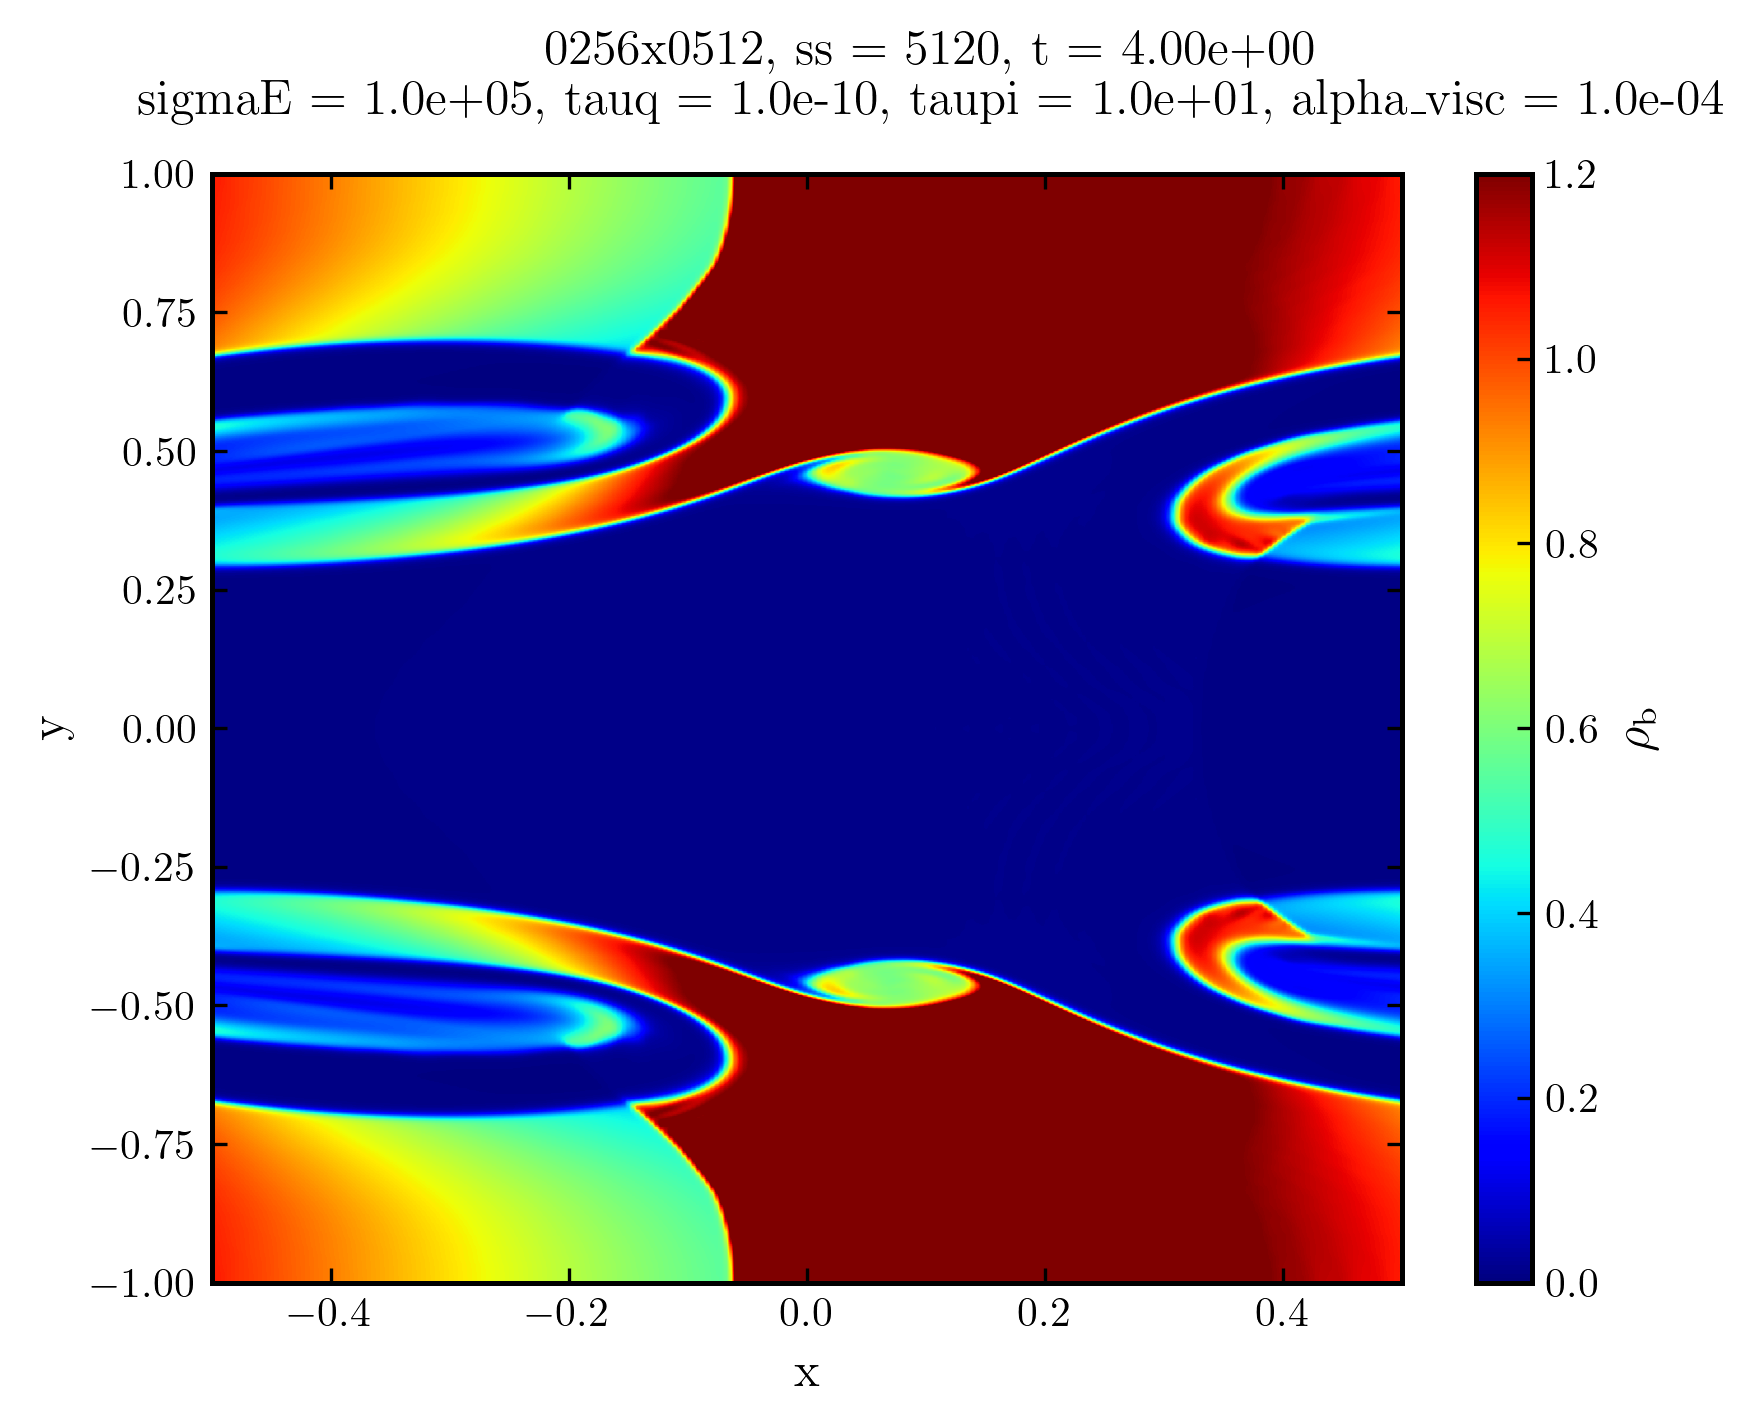
\includegraphics[width=0.8\textwidth]{fig.KHI.png}
  \end{figure}

\end{frame}

\begin{frame}
\frametitle{What Doesn't Work: Viscous, Resistive}

  \begin{figure}[htb!]
    \centering
    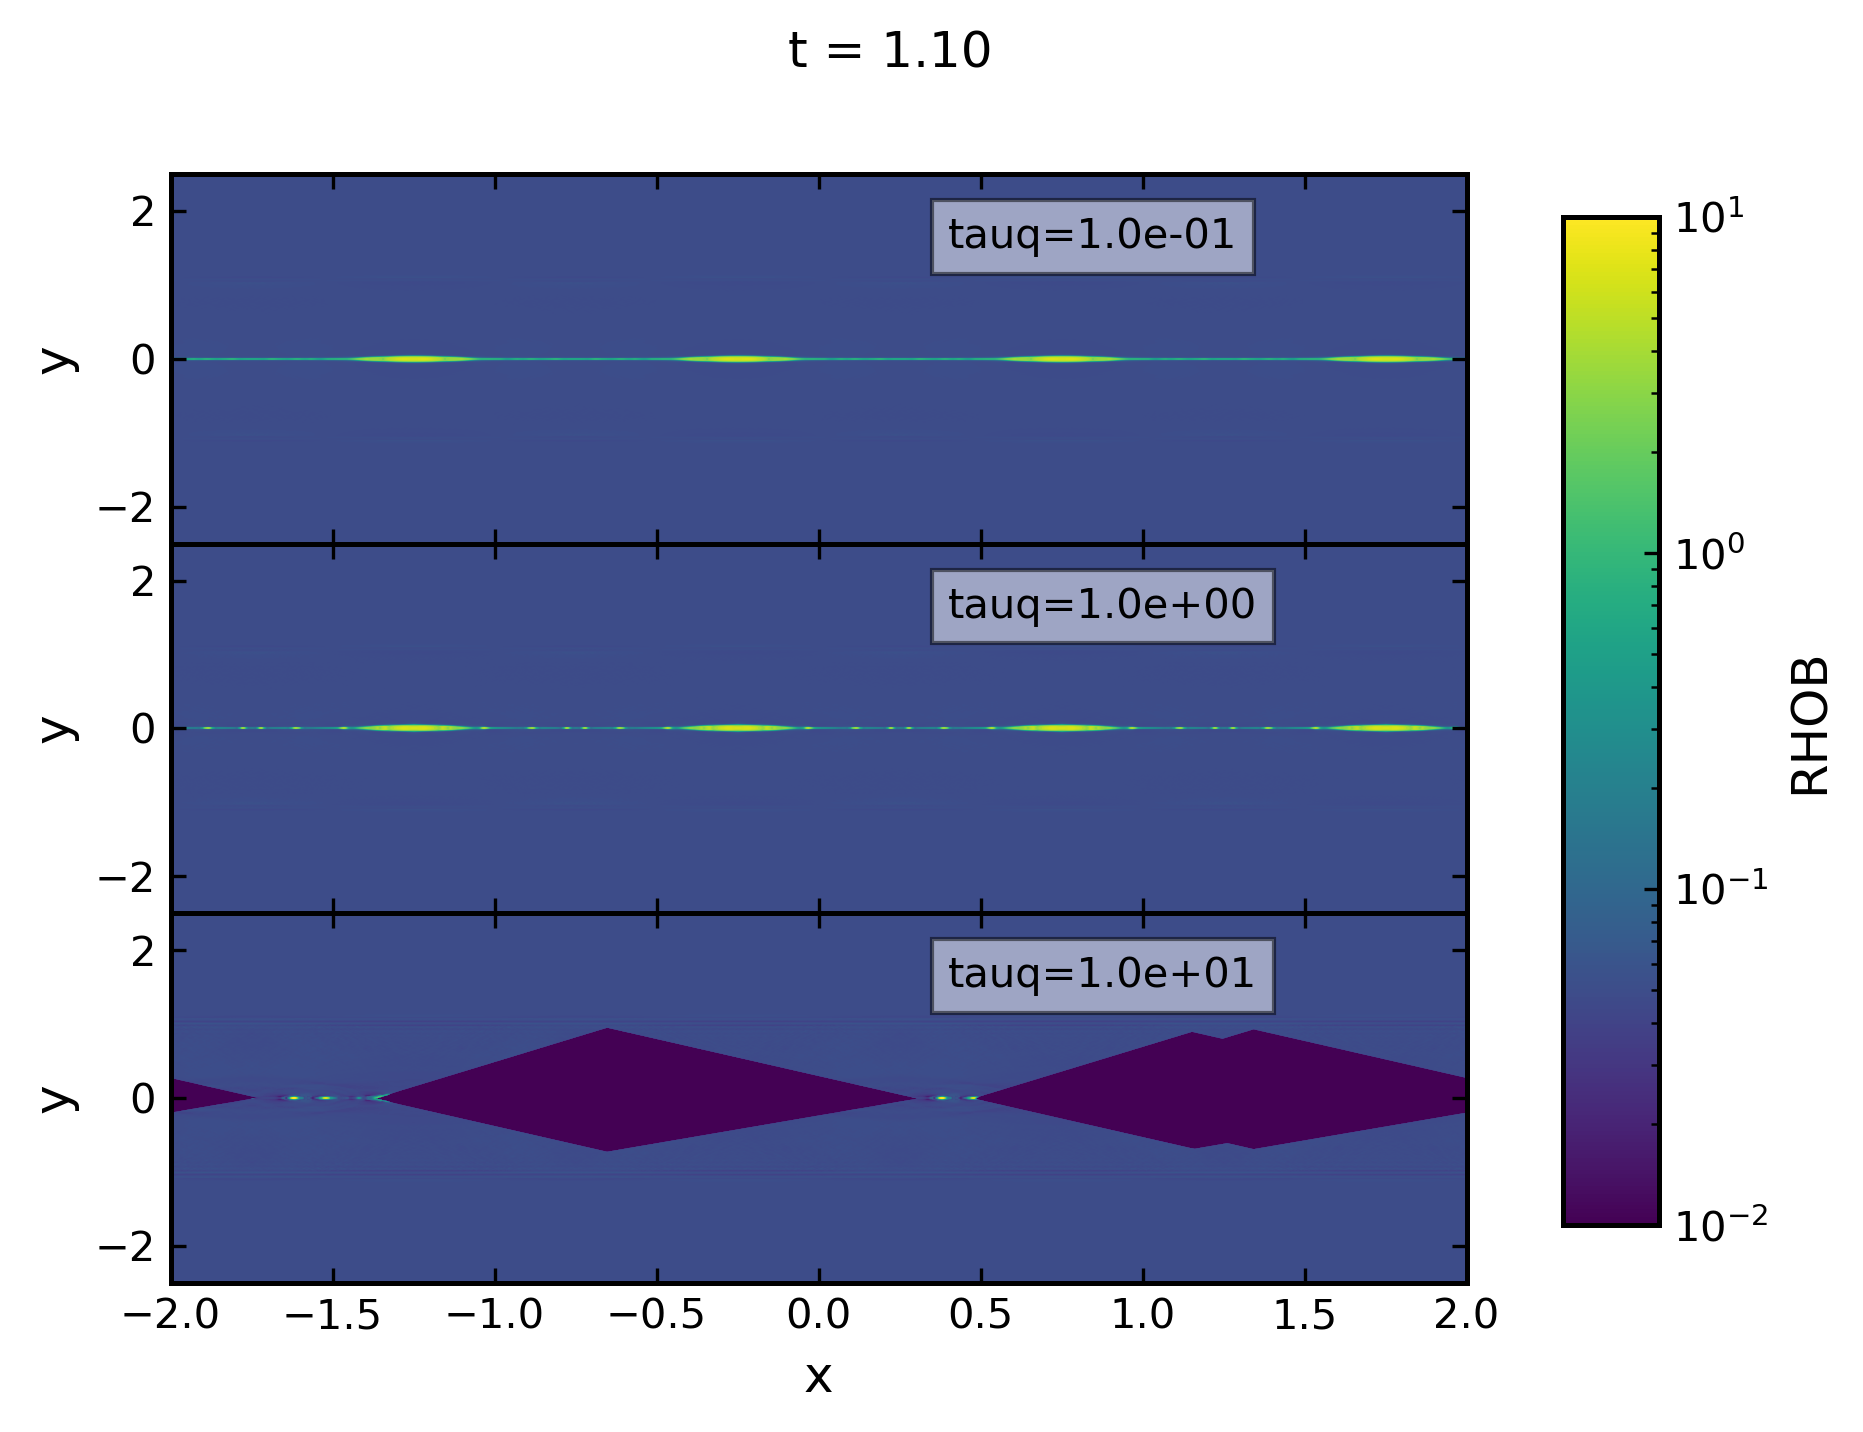
\includegraphics[width=0.8\textwidth]{fig.HarrisSheet.png}
  \end{figure}

\end{frame}

\begin{frame}
\frametitle{Tried So Far}

  \begin{itemize}
    \item Setting floors
    \item Use better initial guess (e.g., ideal solution for $v^{i}$)
    \item Iterate over different variables (e.g., Poynting flux, presssure,
          $1/(h\,W)$)
  \end{itemize}

\end{frame}

\begin{frame}
\frametitle{What to Try Next?}

  \begin{itemize}
    \item Check if $e<0$ with zero heat flux; if so, add energy
    \item If $e>0$ without heat flux and $e<0$ with heat flux, then check $T$
    \item If $T$ is bad, define $q^{\nu} = q^{\nu}\left(q^{*},e\right)$;
    else, limit heat flux
  \end{itemize}

\end{frame}

\begin{frame}
\frametitle{Summary/Future Work}
  \begin{itemize}
    \item
      Developed solver for visco-resistive MHD equations
    \item
      Shown that the model works and shown the influence of visco-resistivity 
    \item
      Make con2prim algorithm more robust
  \end{itemize}
\end{frame}

\appendix

\begin{frame}
\frametitle{Boltzmann--Vlasov Equation}

  Four-momentum vector: $p^{\mu} = \left( E_{\bs{p}}, \bs{p} \right)^{\mu}$,
  with $E_{\bs{p}} := - u \cdot p$ \newline

  Faraday tensor: $F^{\mu\nu} := u^{\mu} \, e^{\nu} - u^{\nu} \, e^{\mu}
                     + \epsilon^{\mu\nu\alpha\beta} \, b_{\alpha} \, u_{\beta}$
  \newline

  Distribution function: $f = f\left( x, p \right)$

  \begin{equation}
    p^{\mu} \, \p_{\mu} \, f
      + \left( q \, F^{\mu\nu} \, p_{\nu}
      + \Gamma^{\mu}_{~\alpha\beta} \, p^{\alpha} \, p^{\beta} \right)
      \p_{p^{\mu}} \, f = C\left[ f \right]
  \end{equation}
  \cite{most2022}

\end{frame}

\begin{frame}
\frametitle{Moments}

  Moments of Boltzmann--Vlasov equation
  lead to definitions of $N^{\mu}$ and $T^{\mu\nu}_{\mathrm{hydro}}
  + T^{\mu\nu}_{\mathrm{dissipative}}$:

  \begin{equation}
    N^{\mu} := \int \frac{g \, d^{3}p}{\left(2\pi\right)^{3} E_{\bs{p}}} \,
    p^{\mu} \, f
  \end{equation}
  \begin{equation}
    T^{\mu\nu}_{\mathrm{hydro}} + T^{\mu\nu}_{\mathrm{dissipative}}
    := \int \frac{g \, d^{3}p}{\left(2\pi\right)^{3} E_{\bs{p}}} \,
    p^{\mu} \, p^{\nu} \, f
  \end{equation}
  \cite{denicol2019}\newline

  With $p^{\mu} = E_{\bs{p}} \, u^{\mu}$ and
  $f = \left( \exp \left( \left( E_{\bs{p}} - \mu \right) / T \right) \right)^{-1}$,
  these become the hydro part of the ideal magnetohydrodynamics equations
  and $T^{\mu\nu}_{\mathrm{dissipative}} = 0$

\end{frame}

\begin{frame}
\frametitle{Bibliography}

  \Fontvi
  \bibliography{main.bib}

\end{frame}

\end{document}
%------------------------------------------------------------------------------%
